\chapter{Dynamic 3D Object Insertion}\label{chp:ObjectLoading}

In order to realise the insertion of a 3D object from a \acs{CAD} file, a plug-in with this functionality was developed called CAD Runtime Importer (\acs{CRI}). Alongside it a standalone Unreal prototype project, named CAD Runtime Presenter (\acs{CRP}), was made that incorporates \acs{CRI} in order to demonstrate how it can be used for a multi-user desktop and VR environment. The whole mechanism can be split into three major sections: opening and parsing the files, generating the objects and lastly user interaction with said objects. How all of this was implemented and what sort of advantages and disadvantages these approaches have will be discussed in this chapter.
%%%%%%%%%%%%%%%%%%%%%%%%%%%%%%%%%%%%%%%%%%%%%%%%%%%%%%%%%%%%%%%%%%%%%%%%%%%%%%%%%%%%%%%%%%%%%%%%%%%%%%
\section{Loading and Parsing CAD Files}
\subsection{File Loading and Sharing}
The first step in creating an object in runtime is opening the desired file and getting the required data from it in runtime. As Unreal Engine is written in C++, it is not surprising that opening up a file is not too much of an issue. What makes this simpler is the fact that Unreal also offers this in their FileHelper class with the functions `LoadFileToString()' and `LoadFileToArray()'. The first function can load a text file into a string, while the other loads binary files into an array of bytes. This is only directly available in C++, therefore it had to be exposed to Blueprints. As this functionality is more of a utility, it is not the best idea to attach it to a specific object. For such purposes, Unreal offers Blueprint Function Libraries\cite{bib:UEBFL}. This is just a special type of Unreal C++ class in which only static functions can be defined. These functions then become available to be used in any Blueprint without needing any instanced objects.\\
Something that is slightly more complicated is choosing the file. Here Unreal does technically offer the ability to open a file dialog but this is a strictly developer only module and can not be used in finished products\cite{bib:DeskPlat}. Neglecting that, it would not work in VR so a separate solution would be needed anyway. Due to this a file picker in CRP's UI had to be written. The end result of that can be seen in Figure \ref{fig:FilePicker}. The design is simple but offers all the necessary functionality, especially as it is compatible with VR and only displays supported file formats.\\

\begin{figure}[htpb]
	\centering
	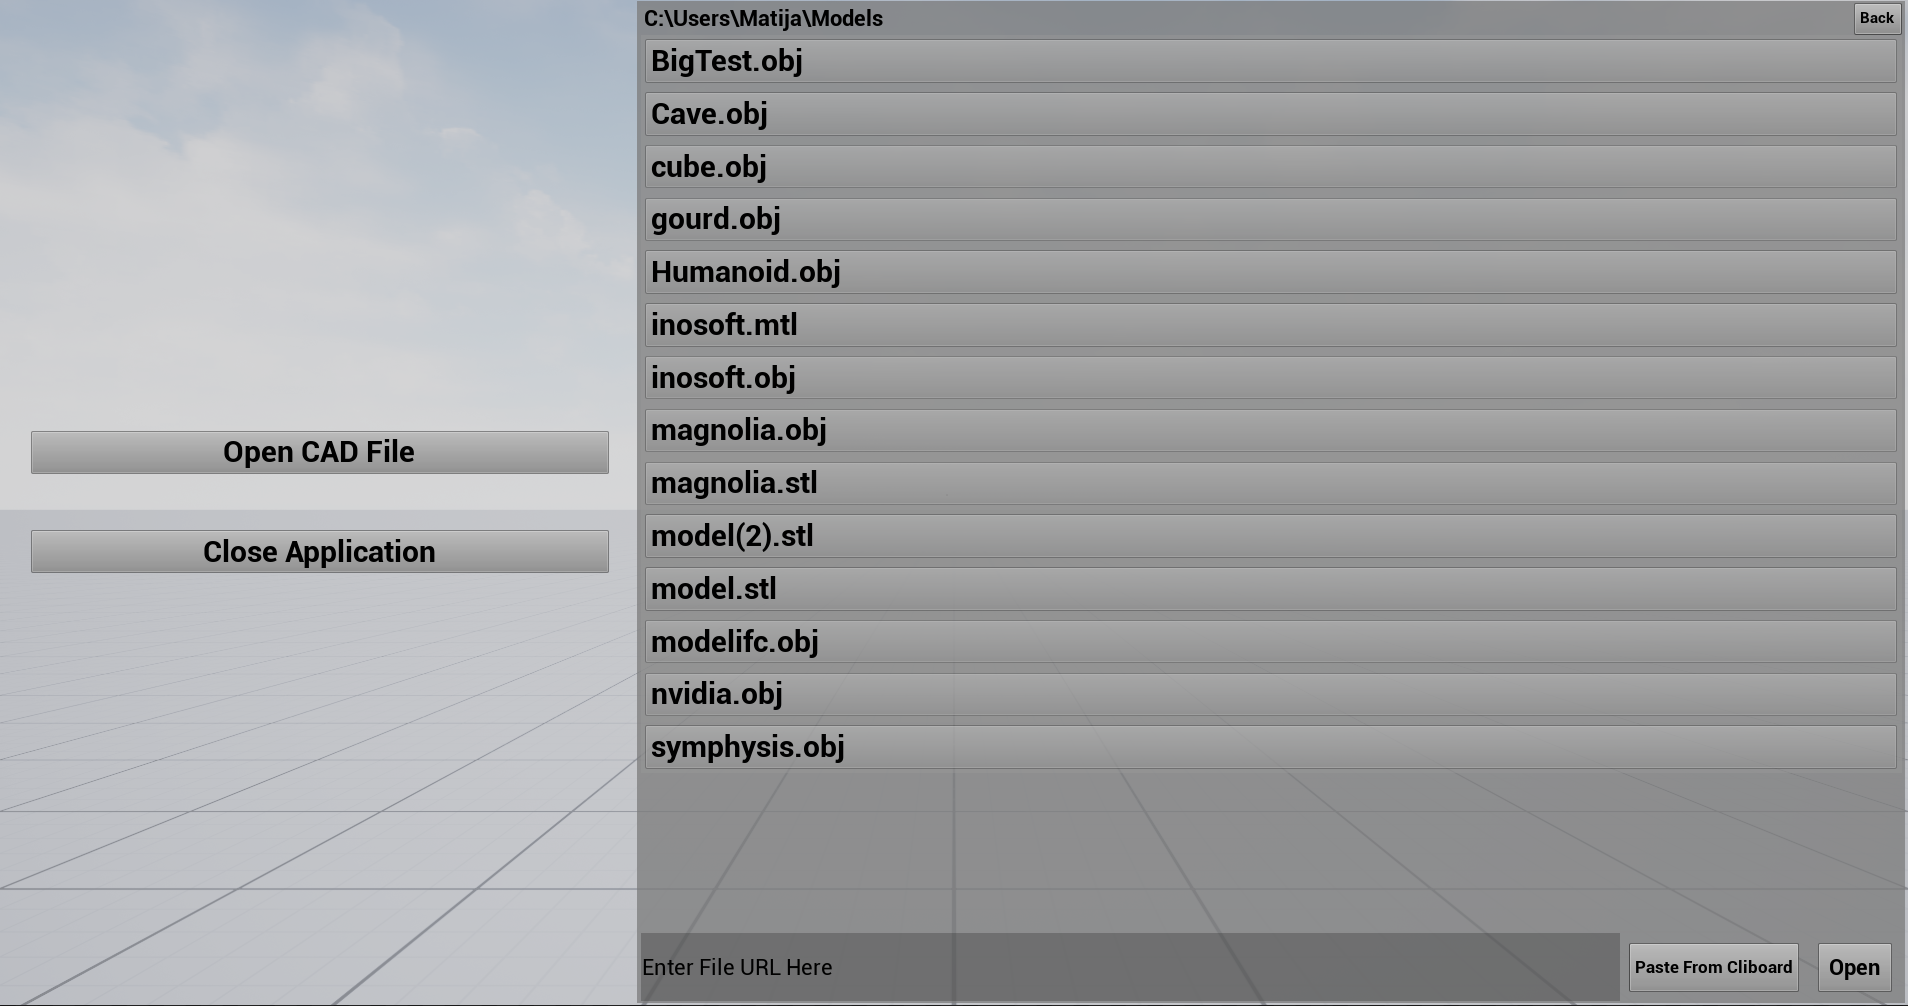
\includegraphics[width=0.9\textwidth]{fig/FilePicker2.png}
	\caption[CAD Runtime Presenter File Picker]{File Picker for CRP\protect}
	\label{fig:FilePicker}
\end{figure}

For a single user this would be enough, they could choose a file and then it could be parsed for object generation. Complications arise once there are multiple users involved. If a user were to open a file in such a scenario, the object would appear only in the world of that user and not for other users or even on the server. This could cause many issues since the client's world would not match server's, which is the authoritative instance. The problem lies in the fact that the new object needs to be created on every client and on the server. In order for that to happen, every machine needs access to the required data, not just the client who has the file available on their machine.\\

One way of sharing this data is saving it in a replicated variable and having it handled by the automatic replication system. This does work but it has one fatal flaw which makes using it not viable. That is the size limit of replicated variables. The size limit for arrays is 64 kilobytes and for strings it seems to be the same. For smaller files this would be a perfect solution, however \acs{CAD} files tend to be too big for it.\\
So instead, this problem was solved by having the file be uploaded to a server and then be downloaded by the rest of the clients and the server. For such purposes, Unreal offers the HTTPModule interface, which uses the popular and powerful libcurl library, to create \acs{HTTP} requests\cite{bib:UELibC}. A file could then be uploaded using a POST request and downloaded using a GET request. For this purpose, a simple file server which can handle such requests was written in python. The only problem is that the clients and server need to know where and what file was uploaded in order to make the correct request. This is where replication becomes useful. The client that uploads the file can tell the server where it was uploaded - through a replicated string - which is most likely to be within the size limit. The server can propagate that information to the rest of the clients, which then make the GET requests.\\
For most users, only the link to the file matters. This means that the client that wants to open a file does not need to have it locally on their machine. Instead, they can input a link to a service like Dropbox or Google Drive and have everyone download those files. The UI for that is also part of the file picker and can be seen at the bottom of Figure \ref{fig:FilePicker}.\\
There are other libraries and plug-ins that could be used to enable file sharing with more complicated protocols, but that was not necessary for this prototype project. The HTTPModule is simple to use while offering all the needed functionalities and avoids having to rely too much on third-party libraries.
%%%%%%%%%%%%%%%%%%%%%%%%%%%%%%%%%%%%%%%%%%%%%%%%%%%%%%%%%%%%%%%%%%%%%%%%%%%%%%%%%%%%%%%%%%%%%%%%%%%%%%
\subsection{Parsing Wavefront OBJ and STL}

Once every instance of the program has the desired file, the next step can begin which is parsing the data. What data is available and how it is stored can vary heavily from format to format. Generally, they will all have the vertices that define the mesh but outside of that colour, material or anything else is not guaranteed. This is the case because \acs{CAD} formats tend to be highly specific for their fields, as well as proprietary for the \acs{CAD} software they were developed for. This makes supporting many \acs{CAD} formats difficult, especially those that are not well documented or do not have publicly available documentation. Considering the scope of this project, spending too much time writing parsers for as many formats as possible was not feasible.\\
Instead, the decision was made to use well-known and widely-supported formats, like OBJ and STL. One of the biggest benefits of this approach is the already existing support that these formats have. Many \acs{CAD} softwares support exporting to one of these and even if they do not, there are probably tools with which the files can be converted. This saved a lot of time during development, as only a few parsers had to be written. For those that had to be implemented, the process was fairly simple due to all of the existing resources on the formats.

\subsubsection{Wavefront OBJ}

Wavefront OBJ, or simply OBJ, is a geometry definition file format developed by Wavefront Technologies for their Advanced Visualizer animation packages\cite{bib:OBJ}. It is a neutral, open-source format which has been widely adopted and has good import and export support from almost all \acs{CAD} software.\\
Another reason why OBJ was chosen, is the fact that it can be read directly through any text editor. This helped significantly in the early stages of development where the primary goal was to prove that the concept worked. Being able to see and read the data made it simpler to write a parser, as well as making it easier to comprehend what was happening with the data at later stages.\\
\begin{table}[htbp]
	\centering 
	\scalebox{0.889}{
		\begin{tabular}{lll}
			\toprule \textbf{Tag} & \textbf{Example Value} & \textbf{Definition} \\
			\bottomrule
			v & 0.2 0.3 0.5 & 3D Vector representing 3D Vertex \\
			vn & 1.0 0.5 0.0 & 3D Vector representing 3D Normal \\
			vt & 0.5 0.25 & 2D Vector representing Texture Coordinate\\
			f & 1/1/2  2/2/5  3/3/5 & Polygonal Face made from Vertices, Normals and Textures\\
			usemtl & Stone & Defines what Material should be used for following Faces\\
			g & Door & Defines a polygon group\\
			\bottomrule
	\end{tabular}}
	\caption[ObjTypes]{Relevant types in OBJ format}
	\label{tab:ObjTypes}
\end{table}

The format represents 3D geometry in the form of vertex positions, vertex normals, texture coordinates, polygonal faces and groups of faces. These geometries can also use materials indirectly by referencing materials defined in a separate \acs{MTL} file. Every entry in an OBJ file is represented through a single line, starting with an identifying tag followed by the value of the entry. What these entries can look like is represented in Table \ref{tab:ObjTypes}.
In order to parse their values, most of the entries can be regarded one-by-one. Vertices, normals and texture coordinates are vectors and can be saved in separate vector arrays in the order in which they appear. How these values are used is explained Chapter \ref{chp:Generating}.\\
Faces, materials and groups are more complicated as they define how the rest of the data is put together to make the object. A face represents a polygon defined through lists of vertex, texture and normal indices in the format "vertexIndex/textureIndex/normalIndex", as can be seen in Table \ref{tab:ObjTypes}. It is important to note that these are the indices of the values and not the values themselves. Also, the indices for vertices, texture coordinates and normals are separate and based on when the entry was defined in the file starting with one. So, both a vector and normal can have their respective index be one. The polygons tend to be triangles but can also have more sides. This is not ideal because generating meshes only supports using triangles. However, there is a simple way to solve this. The vertices are listed in an anticlockwise order, therefore any polygon can be represented through a triangle fan, as is shown in Figure \ref{fig:TriangleFan}. Thus, faces that define polygons with more than 3 edges are replaced through multiple triangular faces.

\begin{figure}[htpb]
	\centering
	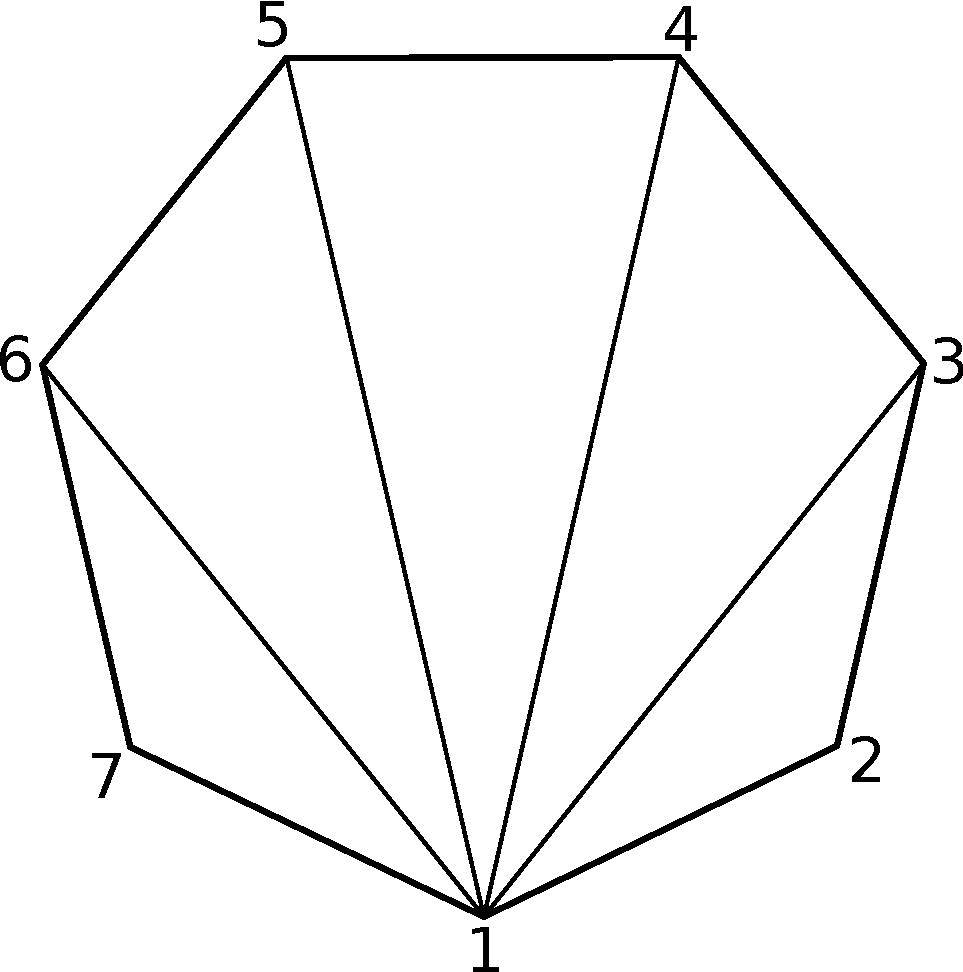
\includegraphics[width=0.3\textwidth]{fig/TriangleFan.pdf}
	\caption[OBJ Polygon to Triangle Fan]{Polygon represented through a Triangle Fan\protect}
	\label{fig:TriangleFan}
\end{figure}

A group determines what faces are combined in order to make a component of the larger object. The ``usemtl" tags tells what material should be used on the following faces and it is used until the next tag appears. The actual materials are defined in an \acs{MTL} file, which works similarly to OBJ, however with different tags and values\cite{bib:MTL}. Some of the more important entries can be seen in Table \ref{tab:MTLTypes}. This \acs{MTL} file of course also needs to be shared to every client. The values themselves are saved in a map, where the keys are the material names and the values are arrays of the values.

\begin{table}[htbp]
	\centering 
	\scalebox{0.889}{
		\begin{tabular}{lll}
			\toprule \textbf{Tag} & \textbf{Example Value} & \textbf{Definition} \\
			\bottomrule
			newmtl & Stone & Defines the name of a new Material\\
			Ka & 1.0 1.0 1.0 & Ambient colour\\
			Kd & 0.0 0.0 0.0 &  Diffuse Colour\\
			Ns & 1.0 & Specular Exponent\\
			d & 0.5 & Transparency\\
			
			\bottomrule
	\end{tabular}}
	\caption[MTL Types]{Example types in MTL format}
	\label{tab:MTLTypes}
\end{table}

As the information of these values heavily relies on each other, they needed to be combined and saved in an array where every entry represents one Component of the whole object. The entry consists of the face values and marks where materials need to be switched.\\
The only major problem with OBJ is that the coordinates do not have units, meaning they can not be scaled to properly represent the designed size. Instead, everything is scaled with the same factor, so that at least the scales between objects made in the same scene stay the same. Also, the created objects can later be scaled by users to better resemble the desired size.

\subsubsection{STL}
STL is a file format native to the \acs{CAD} software created by 3D Systems in 1987\cite{bib:STL}. The format has gained a lot of support in many different software packages, especially for 3D printing software where it is one of the default formats. STL files only describe the surface geometry of a three-dimensional object without any additional information about colours, materials or groups. The geometry is described in raw, unstructured triangles defined by a normal and three vertices. The way a triangle is defined in the file is shown in Figure \ref{fig:STLFormat}. 
\begin{figure}[htpb]
	\centering
	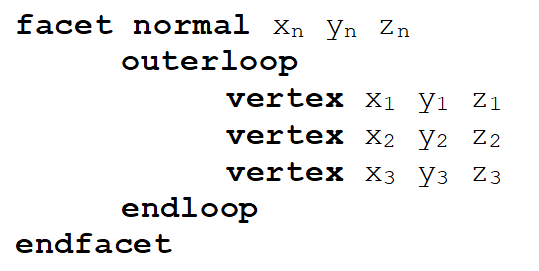
\includegraphics[width=0.35\textwidth]{fig/STLFormat.png}
	\caption[STL Triangle facet]{A triangle facet represented in STL\protect}
	\label{fig:STLFormat}
\end{figure}

While the structure suggests that there are multiple possibilities for loops, the facets can only be triangles. In order to represent a full model, the triangles are simply listed one after the other. While parsing it, the vertices and normals are saved in arrays and faces are generated to define what vertices make up the triangles. This is important for generating the mesh later. While it is a simpler format compared to OBJ, it is excellent when only the shape is relevant. It does unfortunately suffer from the same scaling problems as OBJ and that is handled in the same way as well.\\
Overall, with these two formats the majority of the most common and well-known \acs{CAD} formats are covered. Ideally more formats would be covered and specific parsers for every format would be written to get the most accurate results, but for the limitations of this project, this was a very practical solution.

%%%%%%%%%%%%%%%%%%%%%%%%%%%%%%%%%%%%%%%%%%%%%%%%%%%%%%%%%%%%%%%%%%%%%%%%%%%%%%%%%%%%%%%%%%%%%%%%%%%%%%%%%%%%%%
\section{Runtime Mesh Generation}\label{chp:}

After the files have been parsed and the needed data was extracted, the actual process of creating a new 3D object starts. For that, a way to tell Unreal to generate a mesh is required and it does in fact support such a feature in the form of so-called Procedural Mesh Components(\acs{PMC})\cite{bib:UEPawn}. These Components can be created in runtime by giving them the required mesh data and letting them generate themselves. In the first phases of this project, it was explored as to how viable using these Components were, seeing as they initially seemed to be exactly what was needed. Getting it to function took some time, mostly due to Unreal Engine's generally bad documentation, but the first results with small objects were quite promising. Unfortunately, problems started to arise with larger objects where the performance would drop significantly or Unreal Engine would simply crash. The reason for this lies within \acs{PMC} itself. As the name implies, these Components are supposed to be generated by some form of procedure which generally will not create nearly as many vertices as a large \acs{CAD} file can. On top of that, the underlying architecture for a real procedural system for expensive geometrical operations would be quite different to that of a runtime gameplay framework \cite{bib:ProcProb}. \acs{PMC} is also a relatively late addition to Unreal Engine, first appearing in version 4.8 in 2015. Even though it is designed for a quite similar purpose, it is different enough that it could not be used.\\
Due to this, a different method of getting Unreal to generate meshes had to be found and during this time the most important question for this project came up. Does Unreal not already support runtime mesh generation? Let us say, as an example, there was an Actor that had a static mesh attached to it. Unreal could spawn in this new Actor without a problem. So, should it not be able to create such an Actor from data parsed from a file?\\
A definitive answer for that question could not be found, but through some research a few speculations could be made. The biggest reason for this probably stems from the main purpose of Unreal Engine. Unreal has always and will probably always be a video game engine. As such, it is designed and optimized for scenarios that happen in video games. In a game, every asset and model is carefully crafted and placed in a level. These objects are already known to the game and are packaged within it in an optimized state. The game knows exactly what to do with these and where to load them. That is a part of the core functionality of Unreal. However, it is not exposed directly to a developer because adding externals models to a game is not generally required. Why should a game depend on the user having some specific type of file to load? Those need to be within the game itself. Not to mention the problems and security issues an external file could cause.\\
Another factor that comes into play, are the hardware limitations that existed throughout most of Unreal's lifespan. Computers and gaming consoles were not always as powerful as they are now, especially consoles tend to be very underpowered machines. As such, a lot of work went into optimizing games, so that they would run smoothly on their target platforms. Even nowadays with modern systems that are much faster, optimization is a big part of game development. Especially important, is managing what is loaded in and when, as the systems can have limited memory. Some games will use a loading screen to hide the loading, other games might use a gameplay sequence that slows down the player so that the game has time to load in the next assets. There are even games that would restart the console they were running on, without letting the player know, when the memory was full\cite{bib:Morrowind}. How these assets were stored also played a big role. Some games would use the same asset but with different colours to save space or some games saved the same asset multiple times so it could be accessed from storage quicker. \acs{CAD} files on the other hand tend to be rather big and just creating the files is already a demanding job, which requires good hardware. Due to all of this, the idea of just creating a new external mesh using Unreal's functionality is not of value to game development and is not directly available.\\
However, Unreal is not just a game engine any more. As already mentioned, it has gained popularity in various fields and those have very different demands compared to games. This has led to many new additions to Unreal, most importantly Datasmith. Datasmith is a set of tools and plug-ins developed by Epic Games with the goal of streamlining the process of importing \acs{CAD} files into the engine during development\cite{bib:DSDoc}. It is a relatively new addition to Unreal as it was first released around 2016. \acs{CAD} objects are very different to objects used in game development, they focus on creating geometry for manufacturing and production, while game objects are more focused on looking a certain way and being optimized. Due to this, it is clear that this addition is not meant for game development. However, it was not until August of 2021 with the release of Unreal Engine version 4.27, which brought the Datasmith Runtime plug-in, that Datasmith gained the ability to import meshes in runtime\cite{bib:DSRunDoc}. This plug-in, as it is still very new, is in beta and is still being worked on. Most importantly it shows that with access to the mesh generation functionality of Unreal, it is possible to create meshes from external data in runtime.\\ 

However, the demand for such a functionality has existed for a lot longer and Unreal's existing solution with \acs{PMC} was not good enough. This led to the development of a few plug-ins for it, including Runtime Mesh Component (\acs{RMC}). \acs{RMC} is a third-party plug-in developed by TriAxis-Games that exposes the mesh generation capabilities of Unreal in a much more efficient and feature-rich way compared to \acs{PMC}\cite{bib:RMC}. It promises 50-90 \% lower memory usage and 30-100 \% lower render thread CPU time compared to \acs{PMC}. These claims were checked and the results do match the expected improvements. It is also completely free and has been used in many projects even in larger companies \cite{bib:RMC}. This is why it was finally decided to use \acs{RMC} for the purposes of this project. While ideally this project would not need to rely on a separate plug-in, trying to recreate what is available with \acs{RMC}, which has been around for more than 6 years and has had more than 40 contributors, is not a feasible endeavour. Instead, in order to create something that could truly be used and would perform well, it is much wiser to use this tool and apply its capabilities for the purposes of generating \acs{CAD} models.

\subsubsection{Generating a CAD Model}\label{chp:Generating}

Before a model can be generated, there needs to be an Actor to which the Components can be attached to. This could be any Actor, even the Player Character, but it makes the most sense to create a specific Actor for these purposes. In the plug-in such an Actor is defined in the CRIObject Blueprint class. Actors of this class are going to be where the values from the parsed files will be stored, as well as the Actors that call the function to generate the new Components on themselves. Due to this, it is possible to generate multiple models at the same time, although doing too many at once is not recommended.\\
In order to spawn in a new Actor of this class, the Unreal `SpawnActor' function can be used. This function just needs to know what class should be spawned and where. The first parameter is easy but the second one has a few more options. Depending on what is needed, all the Actors could be spawned in the same place or a user could enter the coordinates. For the purposes of \acs{CRP}, it was decided that the location of the new Actor is going to be where the user is looking. For this, the user's camera rotation is taken as a forward vector, multiplied by a distance and added to the players location. The distance is based on the size of the spawned object so that collision is avoided but it also is not spawned too far from the user. The spawning process happens as soon as clients start downloading the \acs{CAD} files, so that once the files are parsed, there is a place to save the data. The Actors will be in the world but will not be visible or interactive as they do not have any Components yet.\\
Once all of the data has been saved, flags in the Actor get set in order to notify it that generating can begin. This is done because there is no guarantee that the \acs{CAD} and material file will be downloaded in any specific order. Starting the generating process before all the needed data is there would cause problems. The material flag is also only used if the file uses it and the user specified that it should be created with materials.\\
The whole model is not generated all at once as this could cause the program to stutter or freeze for the duration of the process. This happens because it is running on the same thread as the main thread, which means that nothing is rendered until this process is finished. Instead, each Component gets generated separately from the rest, in the order that they are defined in the file. This is realized through the tick event that Actors can have. A tick event is simply an event that gets called every frame or after some regular interval. As the Components themselves are comparatively small, generating one does not cause a significant performance hit that could freeze the main thread. By doing this, the performance cost of generating the model gets spread across every Component and becomes practically negligible. Another benefit of this is the fact that the Components start appearing one after the other in the world, creating an interesting-looking animation. Ideally, multithreading would be used for even better results but Unreal is rather specific about what can be created and modified in other threads due to its built-in garbage collection\cite{bib:MultiThread}.\\
With every tick the `Generate Mesh Component' function is called and a counter is kept in order to know what Components have already been dealt with. The function is implemented in C++ as the performance is necessary, but in order to call it from Blueprints it was implemented in a Blueprint Function library, just like the file reading function. It could also have been implemented as a native function of the CRIObject class but, as this is supposed to function as a plug-in, it did not make sense to limit it to one specific class. This way the functionality can be used in more ways depending on what the user needs. One such way is implemented in \acs{CRP} and will be demonstrated later.\\
How the function works can be seen in Algorithm \ref{algo:MeshGeneration} which shows the process in a simplified pseudocode.

\begin{algorithm}[htpb]
	\texttt{Input} $Actor, ComponentIndex, Vertices, TextCoords, Normals, \linebreak \null \quad\quad \quad ComponentData, Materials, UseCollision;$\\
	$RMC = new \: CustomRuntimeMeshComponent()$\\
	$RMC.ID = ComponentIndex$\\
	$RMC.AttachTo(Actor)$\\
	$RMC.UseCollision = UseCollision$\\
	$Center = FindBoundingBoxMiddle()$\\
	$RMC.SetRelativeLocation(Center)$\\
	$Vertices.Translate(-Center)$\\
	$RMC.CenterVertex = Center$\\
	$Secitons = GetComponentSections(ComponentData)$\\
	$SectionMaterials = GetSectionMaterials(Materials)$\\
	\texttt{for} $i := 0$ \texttt{to} $Sections.Length$ ~\texttt{do}\\
	\hspace{5mm} $Faces = GetFacesForSection(Sections[i])$\\
	\hspace{5mm} $Material = SetupSectionMaterial(ComponentMaterials[i])$\\
	\hspace{5mm} $RMC.CreateSection(i, Vertices, Faces, Normals, TexCoords, Material)\newline$\\
	
	\caption{Pseudocode for generating a Mesh Component}
	\label{algo:MeshGeneration}
\end{algorithm}

As can be seen, the function takes quite a few inputs but all of those are necessary. The first step is instancing a new Runtime Mesh Component object. In this case it is a slightly customized subclass of \acs{RMC} that contains a more variables that can provide further options. One of those being the index of the Component, which is used when interacting with Components. After that, the Component is attached to the Actor generating it, as it cannot exist in a scene on its own. Based on the user's demands, the mesh can be created either with or without collision. Next, a bounding box is generated from the vertices of the Component and the centre of that box is determined. This is done because when a Component is added to an Actor, its relative location is (0,0,0) so it is in the centre of the Actor. The mesh, on other hand, will be placed where the vertices are. Once the whole mesh is generated, it will look exactly the way it should but there will be problems with certain interactions. Let us take rotation as an example. Since the position of the Component is technically in the centre of the object, rotating it will cause the mesh to rotate around the whole object instead of itself. In order to fix that, the Component is placed where the centre of the mesh will be and the vertices are translated the same amount just in the opposite direction. These two translations cancel each other out, so that the whole mesh ends up looking unchanged. Meanwhile, the position of the Component matches the centre of the mesh, so that rotating and scaling work properly. Alternatively, the Component could be moved and translated in specific ways to simulate such a rotation but this is too complicated and unnecessary. The location of the centre is also saved in the custom class as it is required for some interactions that will be explained later.\\
The Component is then split into sections and the material values for the sections are extracted. An \acs{RMC} can contain one or multiple meshes and these are regarded as sections. In this case, the mesh is split according to the materials, seeing as a section can only use one material. This way a Component can have multiple meshes, instead of having to create a Component for every material change. Lastly, for every section, all the indices defining its faces are saved in one array and the appropriate material for it is set up. In Unreal, a completely new material cannot be created at runtime. Instead, an already existing material is needed as the parent for an instance of a dynamic material. Such a dynamic material can be created during gameplay and the values that define it can be altered as well. There is a slight problem due to the plug-in's current limitations. The materials in Unreal are physically based rendering(\acs{PBR}) materials\cite{bib:UEPBR}, while MTL uses Phong-shaded materials\cite{bib:MTL}. These two ways of rendering are vastly different and there is not one true way of converting between them. That is why the diffuse colour, specular exponent and opacity are used to approximate the appropriate values for the \acs{PBR} material. How well this works depends on what material is supposed to be represented. This is slightly unfortunate, but what is more important is the fact that an appropriate material could technically be created. If a new format, that supports \acs{PBR}, were to be added the whole mesh generating approach would still be the same just with the correct values. Also, two parent material are needed, one for opaque and one for translucent materials because of the way Unreal handles opacity.\\
Finally, the \acs{RMC} takes all of the inputs that it needs and creates a section. This is then repeated for every section of every Component until the whole mesh has finished generating. The model will appear in the world in the position where the Actor was spawned and the result of such a process can be seen in Figure \ref{fig:LoadedModel}.

\begin{figure}[htpb]
	\centering
	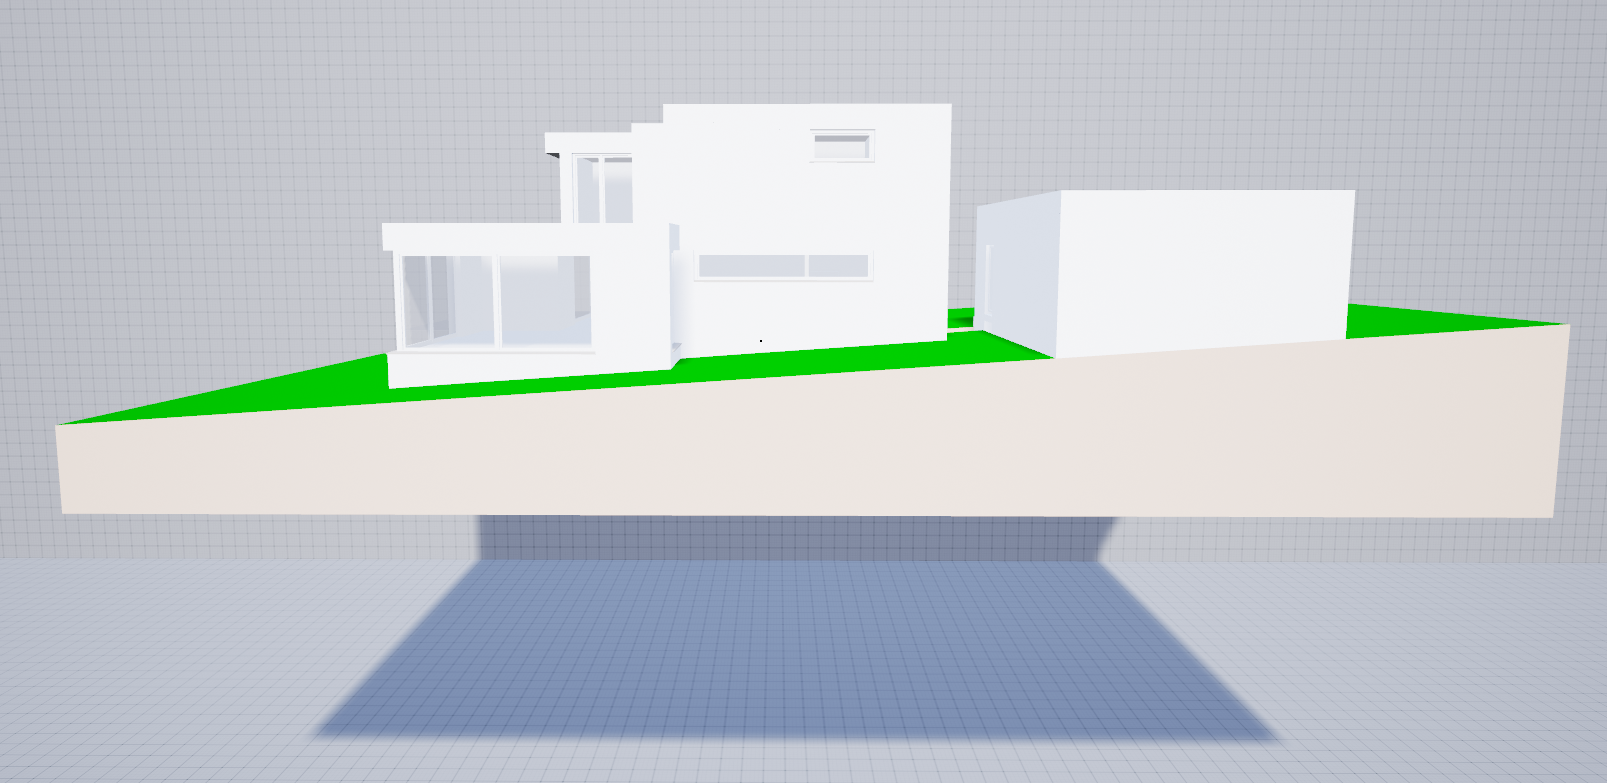
\includegraphics[width=0.65\textwidth]{fig/LoadedModel2.png}
	\caption[Loaded CAD Model in Unreal Engine]{Loaded CAD Model in Unreal Engine\protect\footnotemark}
	\label{fig:LoadedModel}
\end{figure}

\footnotetext{Source of the Model file: Inosoft. All images of this model were made from this file using CRP.}

%%%%%%%%%%%%%%%%%%%%%%%%%%%%%%%%%%%%%%%%%%%%%%%%%%%%%%%%%%%%%%%%%%%%%%%%%%%%%%%%%%%%%%%%%%%%%%%%%%%%%%%%%%%%%%

\section{Object Interaction}\label{chp:ObjectInteraction}
While being able to generate 3D models on its own is very useful, it would be severely limiting if it just stood in a place and the users had no way of doing anything with it. That is why it is important to take a look at how it possible to interact with these objects. There are many ways in which this can be done. The presented solutions are what was implemented in \acs{CRP} to demonstrate some essential and some interesting interactions that can probably find use in most projects.\\
Almost all the interaction was written in the Player Controller, while movement and looking around is handled in the Pawns. This was done because the Pawns have to be different in desktop and VR mode and that would mean writing very similar code in two places. Instead, by having one Controller class and checking what mode is used, this makes for much cleaner code and a more unified experience between the two modes.
\subsection{Grabbing and Translating}

One of the most basic but also most important interactions a user can have with an object is grabbing and moving it around in the world. This is triggered when the user presses the grab button and stays on as long as that button is held. Depending on the mode, this button is either the left mouse button or a trigger on a \acs{VR} controller. When the button is pressed, an \acs{RPC} is called onto the server, where all of the interactions happen. This \acs{RPC} traces a line in the direction that the user is pointing at and checks if any objects get hit by this line. The pointing direction for desktop is where the user is currently looking at, marked for the user as a circular crosshair in the UI. For VR it is simply where the controller, whose trigger was pressed, is pointing at. What this looks like in Blueprints is shown in Figure \ref{fig:LineTracing}.

\begin{figure}[htpb]
	\centering
	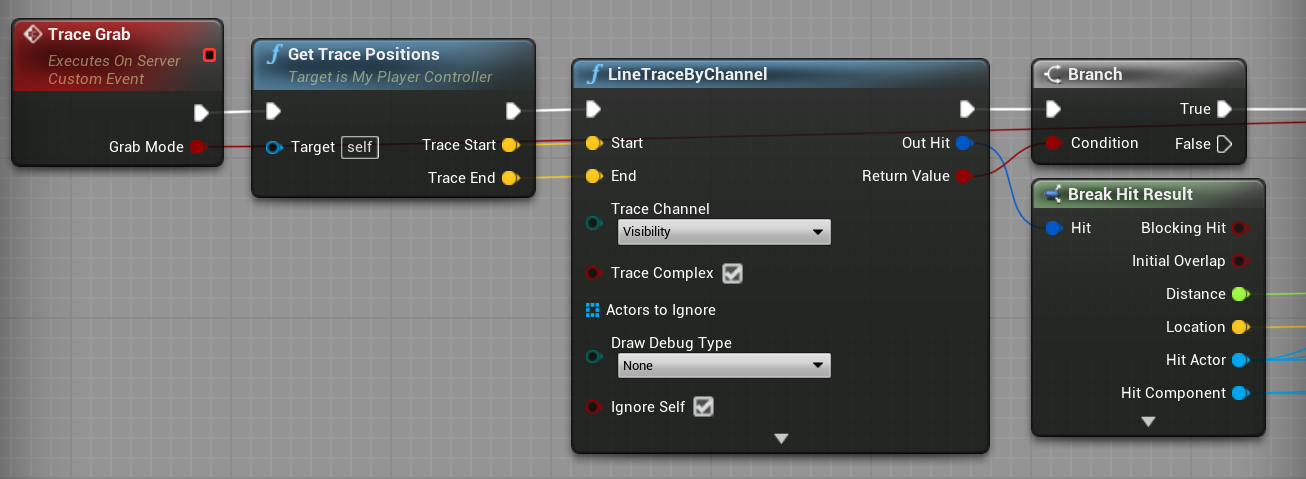
\includegraphics[width=0.8\textwidth]{fig/LineTracing2.png}
	\caption[Tracing Grabs in Blueprints]{Tracing Grabs in Blueprints\protect}
	\label{fig:LineTracing}
\end{figure}

In case there was a hit, a result is created which contains which Actor and Component were hit and where. It is then checked that the correct class of Actor was hit and that the Actor is not already being grabbed. If these checks are passed, a flag on the Actor is set to let other users know that it is currently being grabbed. While this is the case, the Actor will be moved to where the user is pointing at, at the distance that the Actor had when it was grabbed. This location is additionally slightly offset by the position where it was grabbed. If this was not done, once the Actor got grabbed it would instantly move so that the middle of it was where the user is pointing, causing a rather weird looking effect. Instead, the coordinates of where the hit occurred are taken, transformed to the relative coordinate system of the Actor and used as an offset when moving. This way it looks like the user is grabbing the Actor by the part where they intended to. While grabbing, they can also increase and decrease the distance to the Actor as well as rotate it around its z-axis. This is either done through the mouse wheel and two keys on the keyboard or through the stick on the VR controller. As this is all happening on the server and the Actors movement is replicated, it will also be moved in every remote instance. Once the grab button is released, another \acs{RPC} is called that changes the flag on the Actor and ends the grab. Overall, this creates a very intuitive way of grabbing.

\subsection{Scaling and Rotating}

\begin{wrapfigure}{R}{0.39\textwidth}
	\centering
	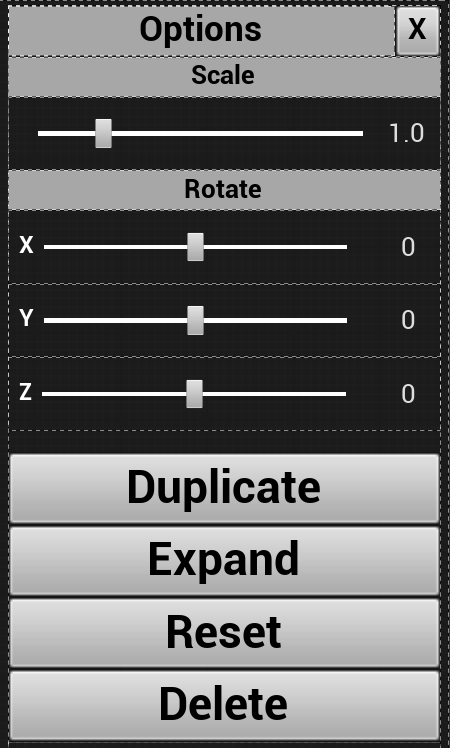
\includegraphics[width=0.30\textwidth]{fig/InteractionMenu2.png}
	\caption[Interaction Menu instead of UI Editor]{Interaction Menu}
	\label{fig:InteractionMenu}
\end{wrapfigure}

The next modes of interaction after translation are scaling and rotation. For these, and the rest of the interactions, a small menu was created for the user-interface which makes these functionalities available. This interaction menu can be seen in Figure \ref{fig:InteractionMenu}. It appears when a user presses the right mouse button or secondary trigger on a \acs{VR} controller while pointing at an Actor. On a desktop window, the menu is located on the right side and is used with a cursor. This cursor captures the mouse movement while the menu is open so that the users view does not move along with it. In \acs{VR}, the menu appears above the other VR controller and is used with the initial controller.\\
The scaling and rotation are done through sliders and the input fields next to them. After one of the values is changed, an \acs{RPC} gets called that tells the server to rotate or scale the selected Actor by the desired amount. This then automatically gets replicated to the other clients.

\subsection{Duplication, Expansion, Resetting and Deletion}

Duplication, as the name says, creates a duplicate of the selected Actor. There are a lot of cases when multiple instances of an Actor are required and instead of having to open the same file for each of those times, it can be done with the click of a button. This uses the fact that the original Actor contains the necessary data, so no further file sharing is needed to create a new one. The new object does not contain the data in order to save on memory. Instead, it has a reference to the original so that in case it also gets duplicated it can point to the necessary data.\\
Expansion aims to give the user a better look at the individual Components and how they make up the whole Actor. This is done by translating the relative positions of the Components in the direction of their centre. By doing this, the Components remain in the relative areas they are supposed to be while creating enough space to differentiate between them.

\begin{figure}[htpb]
	\centering
	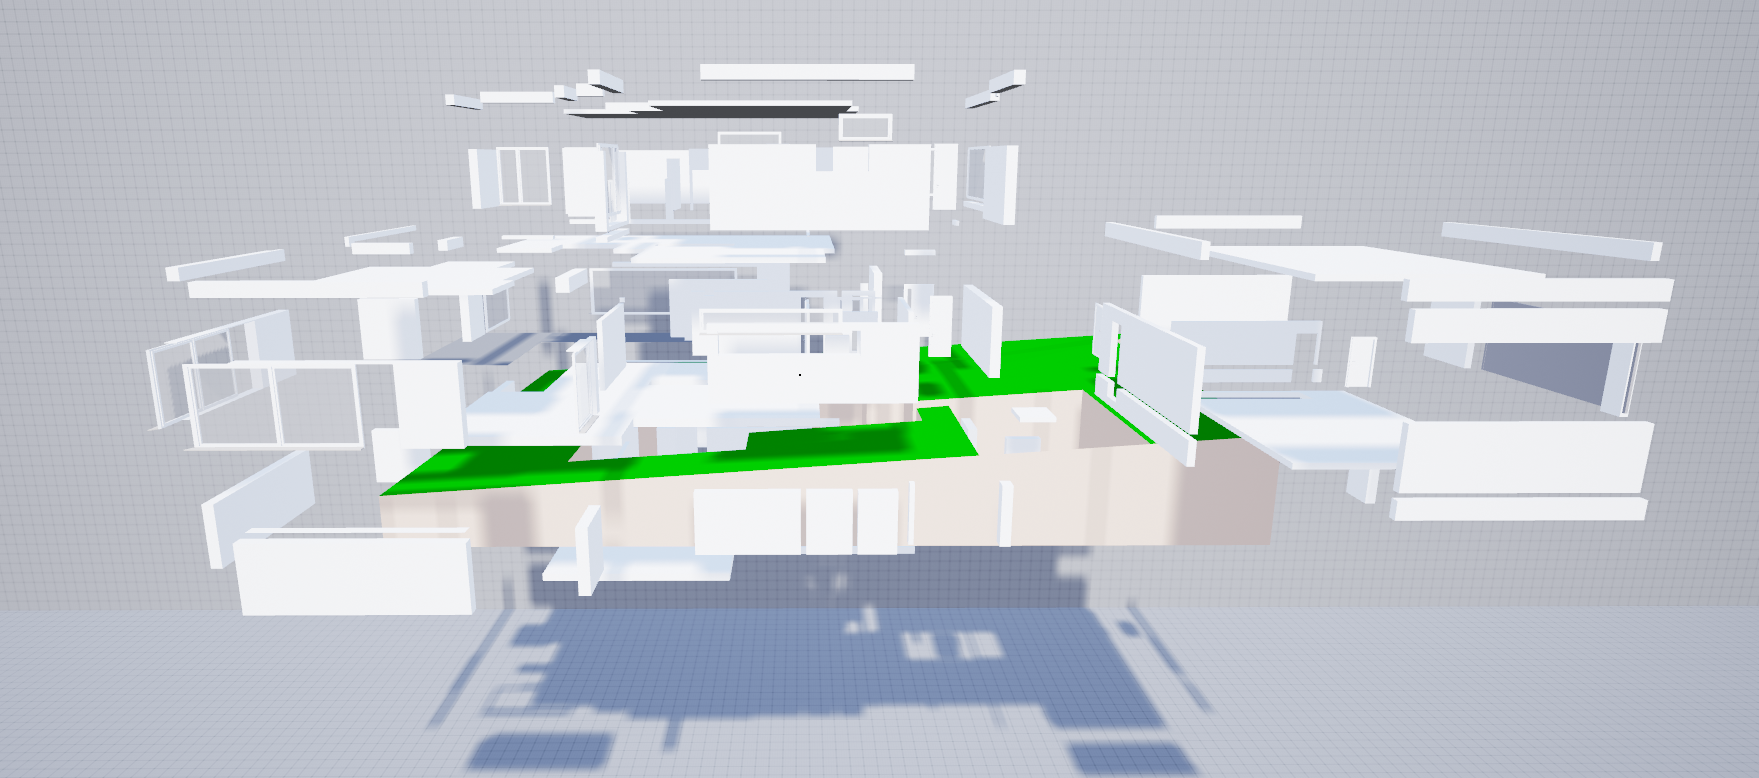
\includegraphics[width=0.8\textwidth]{fig/ExpanedActor.png}
	\caption[Example for an expanded Actor]{Example for an expanded Actor\protect}
	\label{fig:ExpanedActor}
\end{figure}

Resetting is done to undo any sort of changes done to the Actor and put in back into the state it was when it was generated. This means the scaling for every Component is set to 1, the rotation is set to (0,0,0) and the relative location is set to the centre location saved in the Component itself.\\
If objects can be added during runtime, it also make sense to have an option to remove them. Compared to creating, deleting is a lot simpler as Unreal already has functions for that. When deleting an Actor, it is also checked if that is the original instance of it and if there are copies of it in the world. If that is the case, the variables are transferred to a copy and the references for all the of copies are updated.\\

\subsection{Interacting with Individual Components}

While being able to interact with the Actor as a whole is already useful, a lot more could be achieved if users could interact with every Component individually. For that, a separate mode can be toggled with the press of a button. This mode uses the fact that the hit of a line trace also returns what Component was hit. This is used to determine which Component to interact with. However, for the user it might not always be clear which Component is which. So, while the user is in this mode the Component currently being pointed at is highlighted. This effect is achieved through changing the material on the Component with a dynamic material instance and changing it back to its usual material once it is not being targeted. The result of this can be seen in Figure \ref{fig:ComponentHighlight}.\\

\begin{figure}[htpb]
	\centering
	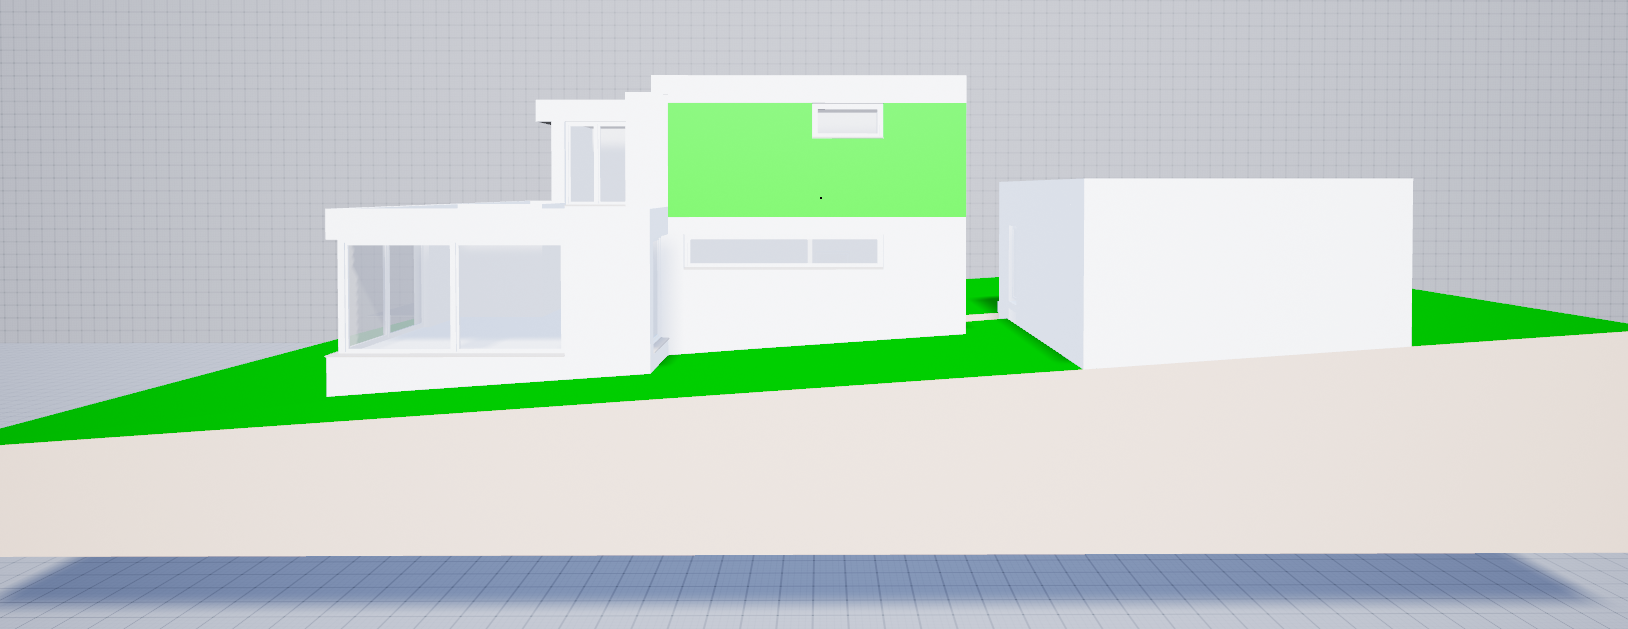
\includegraphics[width=0.8\textwidth]{fig/ComponentHighlight.png}
	\caption[Highlighting a Component in CRP]{Highlighting a Component in CRP\protect}
	\label{fig:ComponentHighlight}
\end{figure}

With this Component, the user can interact in almost all of the same ways they could with an Actor. Only expansion and duplication are not supported. The first one due to it requiring multiple Components and the other one in order to avoid having two identical Components attached to the same Actor.\\
When it comes to translating the Component, a special feature is implemented. Even though the Component can be moved out of its initial space, it is still part of the Actor. If the Actor were to move, so would the Component. Unreal does offer the ability to turn this off through a function called `DetachFromComponent'. While it may seem that the Component now would be independent of the Actor, this is not the case. It purely means that the Component is not moved along with the Actor. Meaning, if the Actor were to be delete, the Component would be gone as well. Truly detaching and reattaching a Component is very finicky and not recommended. Instead, the developed mesh generating functionality can be used to solve this problem. The Component is simply replaced by a new copy of it that is attached to a different Actor. For this Actor, a specific class was made that is designed to hold exactly one Component. This class can call upon the `Generate Mesh Function', as that is a Blueprint Function Library. Therefore, it can generate the specific Component needed by using the index saved in the original. This is done once the Component is released from being grabbed. The original Component is moved away, turned invisible and has its collisions turned off. From the user's perspective, it does not actually look like anything happened but they now have an instance of that Component that can exist completely separately from the original Actor. The user can interact with this newly generated Component in all the ways they usually could. Important to note is that when the reset function is used here, the Component actually deletes itself and returns the original to the way and position it is supposed to be. For the user this just looks like the Component was placed back where it was.\\
Overall, this suite of interactions demonstrates the main ways of interaction and some additional ones that are possible with the newly generated objects. There are definitely countless many more that could be implemented but for the purposes of this prototype, this is quite sufficient. 